\section{Введение}

Хорошо известно (см., например, \cite{coddington}, \cite{krasnoselskii}), что в случае
дифференциальных уравнений условие гладкости правых частей не обеспечивает существования решений задачи с
начальным значением на неограниченном справа интервале. Для существования таких решений в теории обыкновенных
дифференциальных уравнений широко применяется метод односторонней оценки (см., например, \cite{coddington}).
Для дифференциального уравнения в Гильбертовом пространстве $H$ вида
\begin{equation*}
    x' = f(t,х)
\end{equation*}
\noindent одна из простейших оценок такого типа может быть представлена
\begin{equation}
    \label{eq:f_condition}
    \langle f(t,x),x\rangle \leq a \norm{x}^{2} + b
\end{equation}
\noindent Чтобы получить существование решений на неограниченных интервалах в случае уравнений дробного порядка
обычно используют условие сублинейно растущей правой части (см. \cite{kamenskii_aa}, \cite{kamenskii_fpta19},
\cite{kamenskii_m}). Очевидно, что это условие сильнее,
чем (\ref{eq:f_condition}).

В данной работе мы доказываем существование слабых решений такого типа семилинейных дифференциальных включений дробного
порядка в сепарабельном Гильбертовом пространстве, при предположении, что линейная часть включения представлена неограниченным
отрицательно определённым оператором, а нелинейная часть удовлетворяет оценке (\ref{eq:f_condition}). Заметим, что
наша конструкция основана на следующем свойстве дробной производной Капуто функции $x(t)$ в Гильбертовом пространстве:

\begin{equation*}
    {}^{C} D_{0}^{q} \norm{x(t)}^{2} \leq \langle x(t), {}^{C} D_{0}^{q} x(t) \rangle,
\end{equation*}

\noindent которое изучалось в работах: 19, 20, 21.

Работа имеет следующую структуру: в следующем разделе мы представим некоторые предварительные сведения из
дробного нализа и теории уплотняющих многозначных отображений. В третьем разделе мы приводим результат об априорной оценке
решений начальной задачи для полулинейных включений с дробной производной в Гильбертовом пространстве в предположении,
что линейная часть включения отрицательно определена и многозначная нелинейность удовлетворяет односторонней оценке.
Для доказательства этого результата воспользуемся приближёнными методами, онснованными на аппроксимации
Иосиды линейной части включения. В последнем разделе мы применим этот резульат для доказательства существования
слабого решения нашей начальной задачи на каждом конечном интервале и для проверки, что существующие решения ограничены
полуосями.

\section{Основные понятия}

\subsection{Дробная производная}

В этом разделе мы напомним некоторые понятия и определения, которые нам понадобятся в дальнейшем.

Пусть $E$ Банахово пространство над полем вещественных чисел.

\begin{definition}
    Дробной производной Римана-Лиувилля порядка $q \in (0, 1)$ непрерывной функции $g:[0, a] \rightarrow E$ называется
    функция $D_{0}^{q}g$ определённая в следующем виде:
    $$D_{0}^{q}g(t) = \frac{1}{\Gamma(1 - q)}\frac{d}{dt}\int_{0}^{t}(t - s)^{-q}g(s)ds$$
    при условии, что правая часть этого равенства определена корректно.
\end{definition}

Здесь $\Gamma$ это гамма-функция Эйлера $$\Gamma(r) = \int_{0}^{\infty}s^{r-1}e^{-s}ds$$

\begin{definition}
    Дробной производной Капуто порядка $q \in (0, 1)$ непрерывной функции $g:[0, a] \rightarrow E$ называется функция
    ${}^CD_{0}^{q}g$ определённая следующим способом:
    $${}^CD_{0}^{q}g(t) = \Big(D^q(g(\cdot) - g(0))\Big)(t)$$
    при условии, что правая часть этого равенства определена корректно.
\end{definition}

\begin{definition}
    Функция
    $$E_{q,\beta}(z) = \sum_{n=0}^{\infty}\frac{z^n}{\Gamma(qn + \beta)}, \ \ \ q, \beta > 0, z \in \mathbb{C}$$
    называется функцией Миттаг-Леффлера.
\end{definition}

Функция Миттаг-Леффлера имеет следующее асимптотическое представление при $z \rightarrow \infty$:

\begin{equation}
    E_{q,\beta}(z) = 
    \begin{cases}
        \frac{1}{q}z^{\frac{1-\beta}{q}}e^{z^{\frac{1}{q}}} - \sum_{n=1}^{N-1}\frac{z^{-n}}{\Gamma(\beta-qn)} +
        O(|z|^{-N}), \ \ \ |argz| \leq \frac{1}{2} \pi q,\\
        - \sum_{n=1}^{N-1} \frac{z^{-n}}{\Gamma(\beta-qn)} + O(|z|^{-N}), \ \ \ |arg(-z)| \leq (1 - \frac{1}{2}q)\pi.
    \end{cases}
\end{equation}

Обозначим $E_{q,1}$ через $E_{q}$. Обратите внимание, что вторая из приведенных выше формул означает, что в случае
$z = \tau < 0$ и $0 < q < 1$ мы имеем
\begin{equation}
    E_{q}(\tau) \rightarrow 0 \ \text{при} \ \tau \rightarrow - \infty
\end{equation}

Заметим, что из отношений:

\begin{equation*}
    E_{q}(-z) = \int_{0}^{\infty} \xi(\theta)e^{-z\theta}d\theta
\end{equation*}

\noindent и

\begin{equation*}
    E_{q,q}(-z) = \int_{0}^{\infty} q\theta \xi(\theta)e^{-z\theta}d\theta,
\end{equation*}

\noindent где

\begin{equation}
    \xi_{q}(\theta) = \frac{1}{q} \theta^{-1-\frac{1}{q}}\Psi_{q}(\theta^{\frac{-1}{q}}),
\end{equation}

\begin{equation}
    \Psi_{q}(\theta) = \frac{1}{\pi} \sum_{n=1}^{\infty} (-1)^{n-1} \theta^{-qn-1} \frac{\Gamma(nq+1)}{n!} \sin(n \pi q), \ 
    \theta \in \mathbb{R}_{+},
\end{equation}

\noindent следует, что

\begin{equation}
    E_{q}(\tau) > 0, E_{q,q}(\tau) > 0 \ \text{для} \ \tau < 0.
\end{equation}

\begin{remark}
    $\int_{0}^{\infty} \theta \xi_{q}(\theta) d\theta = \frac{1}{\Gamma(q+1)}$,
    $\int_{0}^{\infty} \xi_{q}(\theta) d\theta = 1$, $\xi_{q}(\theta) \geq 0$.
\end{remark}

Рассмотрим скалярное уравнение вида

\begin{equation}
    \label{eq:dxt}
    {}^{C}D^{q} x(t) = \lambda x(t) + f(t), \ \ \ t \in [0, T]
\end{equation}

\noindent с начальным условием

\begin{equation}
    \label{eq:dxt_x0}
    x(0) = x_{0},
\end{equation}

\noindent где $\lambda \ in \mathbb{R}, f : [0, T] \rightarrow \mathbb{R}$ - непрерывная функция. Решением этого уравнения мы
будем называть непрерывную функцию $x : [0, T] \rightarrow \mathbb{R}$, удовлетворяющую условию (\ref{eq:dxt_x0}),
дробная производная ${}^{C}D^{q}x$ которой также непрерывная и удовлетворяет выражению (\ref{eq:dxt}). Известно, что единственное
решение данного уравнения имеет вид

\begin{equation}
    x(t) = E_{q}(\lambda t^{q})x_{0} + \int_{0}^{t} (t-s)^{q-1} E_{q,q}(\lambda(t-s)^{q})f(s)ds.
\end{equation}

Нам понадобится следующее вспомогательное утверждение, являющееся аналогом известной
леммы Гронуолла — Беллмана об интегральных неравенствах \cite{kamenskii_aa}.

\begin{lemma}
    Пусть ограниченная измеримая функция $\omega: [0, T] \rightarrow \mathbb{R}$ удовлетворяет интегральному неравенству
    \begin{equation}
        \omega(t) \leq E_{q} (-\eta t^{q}) \omega(0) + \int_{0}^{t}(t-s)^{q-1} E_{q,q}(-\eta(t-s)^{q})\Big(K + m\omega(s)\Big)ds
    \end{equation}
    где $K \geq 0, \ 0 < m < \eta$. Тогда
    \begin{equation*}
        \omega(t) \leq E_{q} \Big((-\eta+m)t^{q}\Big) \omega(0) + K \int_{0}^{t} (t-s)^{q} E_{q,q} \Big((-\eta+m)(t-s)^{q}\Big)ds.
    \end{equation*}
\end{lemma}

\subsection{Меры некомпактности и уплотняющие многозначные отображения}

Напомним некоторые понятия и факты.

Пусть $\mathcal{E}$ - Банахово пространство. Введем следующие обозначения:

\begin{itemize}
    \item $Pb(\mathcal{E}) = \{A \subseteq \mathcal{E} : A \neq \emptyset \ \text{ограничено}\}$;
    \item $Pv(\mathcal{E}) = \{A \in Pb(\mathcal{E}) : A \ \text{выпукло}\}$;
    \item $K(\mathcal{E}) = \{A \in Pb(\mathcal{E}) : A \ \text{компактно}\}$;
    \item $Kv(\mathcal{E}) = Pv(\mathcal{E}) \cap K(\mathcal{E})$.
\end{itemize}

\begin{definition}
    Пусть $(\mathcal{A}, \geq)$ - частично упорядоченное множество. Функция $\beta : Pb(\mathcal{E}) \rightarrow \mathcal{A}$ называется
    мера некомпактности (МНК) в $\mathcal{E}$, если для каждого $\Omega \in Pb(\mathcal{E})$ выполнено:
    $$\beta(\overline{co}\Omega) = \beta(\Omega),$$
    где $\overline{co}\Omega$ обозначает замыкание выпуклой оболочки $\Omega$.
\end{definition}

Мера некомпактности $\beta$ называется:

\begin{enumerate}
    \item \textit{монотонной}, если для каждого $\Omega_0, \Omega_1 \in Pb(\mathcal{E})$, из $\Omega_0 \subseteq \Omega_1$
    следует, что $\beta(\Omega_0) \leq \beta(\Omega_1)$;
    \item \textit{невырожденной}, если для для каждого $a \in \mathcal{E}$ и каждого $\Omega \in Pb(\mathcal{E})$
    выполняется $\beta({a} \cup \Omega) = \beta(\Omega)$;
\end{enumerate}

Если $\mathcal{A}$ - конус в Банаховом пространстве, МНК $\beta$ называется:

\begin{enumerate}
    \setcounter{enumi}{2}
    \item \textit{регулярной}, если $\beta(\Omega) = 0$ равносильно относительной компактности $\Omega \in Pb(\mathcal{E})$;
    \item \textit{вещественной}, если $\mathcal{A}$ - множество всех вещественных чисел $\mathbb{R}$ с естественным порядком;
    \item \textit{алгебраически полуаддитивной}, если $\beta(\Omega_0 + \Omega_1) \leq \beta(\Omega_0) + \beta(\Omega_1)$ для
    любых $\Omega_0, \Omega_1 \in Pb(\mathcal{E})$.
\end{enumerate}

Следует отметить, что МНК Хаусдорфа подчиняется всем вышеперечисленным свойствам. Другими примерами могут служить следующие
меры некомпактности, определенные на $Pb(C([0, a]; E))$, где $C([0, a]; E)$ - пространство непрерывных функций
со значениями в сепарабельном Банаховом пространстве $E$:

\begin{enumerate}
    \item послойная мера некомпактности:
    $$\varphi(\Omega) = \sup_{t \in [0, a]} e^{-pt} \chi_{E}(\Omega(t)),$$
    где $p > 0$, $\chi_{E}$ - Хаусдорфова МНК в $E$ и $\Omega(t) = {y(t): y \in \Omega}$;
    \item модуль равностепенной непрерывности, определяемый как
    $$mod_{c}(\Omega) = \lim_{\delta \rightarrow 0} \sup_{y \in \Omega} \max_{|t_1 - t_2| \leq \delta} \norm{y(t_1) - y(t_2)}.$$
\end{enumerate}

Обратите внимание, что эти МНК удовлетворяют всем вышеупомянутым свойствам, кроме регулярности. Чтобы получить регулярную МНК
в пространстве $C([0, a]; E)$, мы можем рассмотреть МНК

$$\nu(\Omega) = \bigg( \varphi(\Omega),mod_{C}(\Omega) \bigg)$$

\noindent со значениями в конусе $\mathbb{R}^{2}$ с естественным частичным порядком.

\begin{definition}
    Пусть $X \subseteq \mathcal{E}$ - замкнутое подмножество; многозначное отображение (мультиотображение)
    $\mathcal{F}: X \rightarrow K(\mathcal{E})$ называется полунепрерывным сверху (п.н.с), если прообраз
    $$\mathcal{F}^{-1}(V) = \{x \in X: \mathcal{F}(x) \subset V\}$$
    каждого открытого множества $V \subset \mathcal{E}$ открыто в $X$.
\end{definition}

\begin{definition}
    П.н.с. мультиотображение $\mathcal{F}: \Lambda \times X \rightarrow K(\mathcal{E})$ называется уплотняющим относительно
    МНК $\beta$ (или $\beta$-уплотняющим), если для любого ограниченного множества $\Omega \subseteq X$, которое не является относительно
    компактным, выполняется
    $$\beta(\mathcal{F}(\Omega)) \ngeqq \beta(\Omega).$$
\end{definition}

В более общем смысле, учитывая метрическое пространство $\Lambda$ параметров, мы будем говорить, что п.н.с. мультиотображение
$\Gamma: \Lambda \times X \rightarrow K(\mathcal{E})$ является уплотняющим семейством по отношению к МНК $\beta$ (или $\beta$-уплотняющим
семейством), если для каждого ограниченного множества $\Omega \subseteq X$, которое не является относительно компактным, выполняется

$$\beta(\Gamma(\Lambda \times \Omega)) \ngeqq \beta(\Omega).$$

Пусть $V \subset \mathcal{E}$ - ограниченное открытое множество, $\beta$ - монотонная невырожденная МНК в $\mathcal{E}$
и $\mathcal{F}: \overline{V} \rightarrow Kv(\mathcal{E})$ - $\beta$-уплотняющее мультиотображение такое, что $x \notin \mathcal{F}(x)$
для всех $x \in \partial V$, где $\overline{V}$ и $\partial V$ обозначают замыкание и границу множества $V$.

В таких условиях \textit{топологическая степень}

$$deg(i - \mathcal{F}, \overline{V})$$

\noindent соответствующего векторного мультиполя $i - \mathcal{F}$, удовлетворяющего стандартным свойствам, где $i$ -
тождественное отображение на $\mathcal{E}$. В частности, из условия

$$deg(i - \mathcal{F}, \overline(V)) \neq 0$$

\noindent следует, что \textit{множество неподвижных точек} $Fix\mathcal{F} = \{x: x \in \mathcal{F}(x)\}$ является непустым подмножеством $V$.

Чтобы описать следующее свойство, введем следующее понятие.

\begin{definition}
    Преположим, что $\beta$-уплотняющие мультиотображения $\mathcal{F}_0, \mathcal{F}_1: \overline{V} \rightarrow Kv(\mathcal{E})$
    не имеют неподвижных точек на границе $\delta V$ и существует $\beta$-уплотняющее семейство
    $\mathfrak{H}: [0, 1] \times \overline{V} \rightarrow K(\mathcal{E})$ такое, что:
    \begin{enumerate}
        \item $x \notin \mathfrak{H}(\lambda, x)$ для всех $(\lambda, x) \in [0, 1] \times \partial V$;
        \item $\mathfrak{H}(0, \cdot{}) = \mathcal{F}_0; \ \mathfrak{H}(1, \cdot{}) = \mathcal{F}_1.$
    \end{enumerate}
    тогда мультиполя $\Phi_0 = i - \mathcal{F}_0$ и $\Phi_1 = i - \mathcal{F}_1$ называются гомотопическими:
    $$\Phi_0 \sim \Phi_1$$
\end{definition}

\textit{Свойство гомотопической инвариантности топологической степени} утверждает, что если $\Phi_0 \sim \Phi_1$, то
$deg(i - \mathcal{F}_0, \overline{V}) = deg(i - \mathcal{F}_1, \overline{V})$.

Отметим еще следующее свойство топологической степени, которое нам понадобится в дальнейшем. \textit{Свойство нормализации}.
Если $\mathcal{F}(x) \equiv A \in K(\mathcal{E})$, то

\begin{equation*}
    deg(i - \mathcal{F}, \overline{V}) = 
    \begin{cases}
        1, \ \text{если} \ A \subset V, \\
        0, \ \text{если} \ A \cap \overline{V} = \emptyset.
    \end{cases}
\end{equation*}

\section{Априорные оценки решений}

Пусть $H$ - сепарабельное Гильбертово пространство. Рассмотрим задачу Коши для полулинейного дифференциального включения
дробного порядка в $H$:

\begin{equation}
    \label{eq:cd_0q}
    {}^CD_{0}^{q}x(t) \in Ax(t) + F(t, x(t)), \quad t \in [0, T]
\end{equation}

\begin{equation}
    \label{eq:cd_0q_x0}
    x(0) = x_0,
\end{equation}

\noindent где $0 < q < 1$ и линейный оператор $A$ удовлетворяет следующему условию:
(A) $A: D(A) \subseteq H \rightarrow H$ - линейный замкнутый (не обязательно ограниченный) оператор, порождающий ограниченную $C_0$-полугруппу
${U_A(t)}_{t \geq 0}$ линейных операторов в $H$ и такой, что

\begin{equation*}
    \langle Ax, x \rangle \leq -d \norm{x}^2, \forall x \in D(A)
\end{equation*}

\noindent для некоторых $d > 0$.

Предполагается, что мультиотображение $F: [0, T] \times H \rightarrow K_v(H)$ удовлетворяет следующим условиям:

\begin{enumerate}[start=1,label={F\arabic*)}]
    \item функция $F(\cdot, x): [0, T] \rightarrow K_v(H)$ допускает измеримый выбор для каждого $T > 0$ и $x \in H$,
    т. е. существует измеримая функция $f: [0, T] \rightarrow H$ такая, что что $f(t) \in F(t, x)$ для п. в. $t \in [0, T]$;
    \item мультиотображение $F(t, \cdot): \rightarrow K_v(H)$ п.н.с для каждого $T > 0$ и п. в. $t \in [0, T]$;
    \item для каждого $R > 0$ и $T > 0$ существует функция $m_R \in L^\infty [0, T]$ такая, что из $x \in H, \norm{x} \leq R$ следует
    $$\norm{F(t,x)} \leq m_R(t) \text{ для п. в. } t \in [0, T];$$
    \item для каждого $T > 0$ существует $\mathcal{k} \in L^\infty [0, T]$ такое, что для любого ограниченного множества
    $\omega \subset H$ выполняется:
    $$\chi (t, \Omega) \leq \mathcal{k} (t) \chi (\Omega),$$
    где $\chi$ обозначает МНК Хаусдорфа в пространстве $H$;
    \item существует такое $a \geq 0$, что
    $$\sup_{y \in F(t,x)} \langle y,x \rangle \leq a \norm{x}^2 + G(t), \quad t \in [0, T],$$
    где $G: R_+ \rightarrow R_+$ - локальная $L^\infty$ -функция, т. е. $G|_{[0, T]} \in L^\infty[0, T]$ для каждого $T > 0$.
\end{enumerate}

Из условий (F1) - (F3) следует, что для каждого $T > 0$ мультиоператор суперпозиции
$\mathcal{P}_F: C([0, T]; H) \multimap L^\infty ((0, T); H)$ определяется формулой:

\begin{equation}
    \mathcal{P}_F(x) = \{ f \in L^\infty ((0, T); H): f(s) \in F(s, x(s)) \text{ для п.в. } s \in [0, T] \}.
\end{equation}

\begin{theorem}
    \label{th:c_exist}
    При указанных выше условиях существует непрерывная функция $C: [0, +\infty) \rightarrow [0, +\infty)$ такая,
    что для любого решения $x$ задачи (\ref{eq:cd_0q})-(\ref{eq:cd_0q_x0}), определенного на интервале $[0, T]$,
    справедлива следующая априорная оценка:
    $$\norm{x}_{C([0, T], H)} \leq \mathcal{C}(T).$$
\end{theorem}

\noindent Доказательство этой теоремы представлено в \cite{kamenskii_main}.

\begin{equation}
    \label{eq:C}
    \norm{x(t)}^2 \leq E_q(t)\norm{x_0} + \int_0^t (t-s)^{q-1} E_{q,q}((-d+a)(t-s)^q)G(s)ds
\end{equation}

Правая часть этого неравенства определяет функцию априорной оценки $C$ на интервале $[0, T]$.

\section{Существование решения}

Из теоремы \ref{th:c_exist} можно получить следующий результат о существовании решения задачи (\ref{eq:cd_0q})-(\ref{eq:cd_0q_x0}) на произвольном
интервале $[0, T]$.

\begin{theorem}
    При указанных выше условиях задача (\ref{eq:cd_0q})-(\ref{eq:cd_0q_x0}) имеет слабое решение на $[0, T]$ для каждого $T > 0$.
\end{theorem}

\noindent \textit{Доказательство.} Рассмотрим семейство многозначных интегральных операторов
$\mathfrak{F}: C([0, T]; H) \times [0, 1] \multimap (C([0, T]; H)$, определенное следующим образом:

\begin{equation}
    \label{eq:F_xlambda}
    \mathfrak{F}(x, \lambda) = {z = \mathcal{G}_A (t) x_0 + \lambda \int_0^t (t-s)^{q-1} \mathcal{T}_A (t-s) f(s) ds:
    f \in \mathcal{P}_F (x)},
\end{equation}

\noindent где $\mathcal{P}_F$ - мультиоператор суперпозиции, определённый в (3.3).

Ясно, что каждая неподвижная точка $x_{\lambda} \in C([0, T]; H)$ мультиотображения $F (\cdot, \lambda), \lambda \in [0, 1]$,
является слабым решением задачи

\begin{equation}
    \label{eq:cd_0q_l}
    {}^CD_{0}^{q}x(t) \in Ax(t) + \lambda F(t, x(t)), \quad t \in [0, T]
\end{equation}

\begin{equation}
    \label{eq:cd_0q_x0_l}
    x(0) = x_0.
\end{equation}

Более того, известно (см. \cite{kamenskii_fpta19}, \cite{kamenskii_m}), что семейство (\ref{eq:F_xlambda}) имеет компактные выпуклые значения и уплотняется относительно
МНК $\nu$ в $C([0, T]; H)$ (см. раздел 2). Поскольку мультиоператоры $\lambda F$ удовлетворяют условиям (F1)-(F5) независимо от $\lambda$,
применяя теорему 18, мы заключаем, что существует постоянная $\mathcal{C}(T)$ такая, что все решения задачи
(\ref{eq:cd_0q_l})-(\ref{eq:cd_0q_x0_l}) удовлетворяют условию априорной оценки
$$\norm{x_{\lambda}} \leq \mathcal{C}(T).$$

\noindent Итак, мультиоператоры $\mathfrak{f}(\cdot, \lambda)$ из семейства (\ref{eq:F_xlambda}) не имеют неподвижных точек на границе шара
$\mathfrak{B}$ пространства $C([0, T]; H)$ с центром в нуле радиуса $\mathcal{C}(T) + 1$. Обратите внимание, что диапазон мультиоператора
$\mathfrak{f}(\cdot, \lambda)$ состоит из единственной функции $y(t) = \mathcal{G}_A(t)x_0$, являющейся его фиксированной точкой.

Теперь, применяя гомотопические и нормировочные свойства топологической степени, получаем
$$deg(i - \mathfrak{F}(\cdot, 1), \mathfrak{B}) = deg(i - \mathfrak{F}(\cdot, 0), \mathfrak{B}) = 1$$
что, по свойству существования топологической степени, дает желаемый результат.

\begin{flushright}
    $\square$
\end{flushright}

\section{Ограниченность решений на полуоси}

Полученная априорная оценка (\ref{eq:C}) позволяет доказать следующее утверждение о существовании ограниченных на $[0, \infty)$ решений задачи
(\ref{eq:cd_0q})-(\ref{eq:cd_0q_x0}).

\begin{theorem}
    Предположим, что $d > a$, выполнены условия (F1)-(F5) и функция G из условия (F5) принадлежит пространству $L^r[0, \infty)$,
    где $r > \frac{1}{q}$. Тогда каждое решение задачи (\ref{eq:cd_0q})-(\ref{eq:cd_0q_x0}) ограничено на $[0, \infty)$.
\end{theorem}

\noindent \textit{Доказательство.} В силу теоремы 18 все решения задачи (\ref{eq:cd_0q})-(\ref{eq:cd_0q_x0}) определены на $[0, \infty)$
и удовлетворяют оценке (3.19). Поскольку

\begin{equation*}
    E_q((-d+a)t)\norm{x_0} \rightarrow 0 \quad \text{при} е \rightarrow \infty,
\end{equation*}

\noindent для доказательства теоремы достаточно показать, что выражение

\begin{equation}
    \label{eq:int_ts}
    \int_0^t (t-s)^{q-1} E_{q,q}\Big((-d+a)(t-s)^{q}\Big)G(s)ds
\end{equation}

\noindent ограничено, для $t \in (0, \infty)$.

Пусть при $\tau > T$ справедлива следующая асимптотика для функции $E_{q,q}(\tau)$

\begin{equation*}
    0 \leq E_{q,q}\Big((-d+a) \tau\Big) < \frac{c}{\tau},
\end{equation*}

\noindent где $C$ - постоянная. Тогда при $\tau > T^{\frac{1}{q}}$ имеем следующую оценку:

\begin{equation*}
    0 \leq E_{q,q}\Big((-d+a) \tau^q \Big)| < \frac{c}{\tau},
\end{equation*}

\noindent Для $\tau \leq T^{\frac{1}{q}}$ справедлива оценка $E_{q,q}(\tau^q) \leq M$.

Оценим для больших $t$ выражение (\ref{eq:int_ts}):

\begin{equation*}
    \begin{gathered}
        \left| \int_0^t (t-s)^{q-1} E_{q,q} ((-d+a)(t-s)^{q})G(s)ds \right| \leq \\
        \leq \int_{t-T^{\frac{1}{q}}}^{t}(t-s)^{q-1} E_{q,q} \Big( (-d+a)(t-s)^{q} \Big) \left| G(s) \right| ds + \\
        + \int_0^{t-T^{\frac{1}{q}}} (t-s)^{q-1} E_{q,q} \Big( (-d+a)(t-s)^{q} \Big) \left| G(s) \right| ds = I_1(t) + I_2(t)
    \end{gathered}
\end{equation*}

\noindent Пусть $\frac{1}{q} + \frac{1}{r} = 1$, тогда по неравенству Гёльдера

\begin{equation*}
    I_1(t) \leq \left( \int_{t-T^{\frac{1}{q}}}^t (t-s)^{p(q-1)M^p ds} \right)^{\frac{1}{p}}
    \left( \int_{t-T^{\frac{1}{q}}}^t \left|G(s)\right|^r ds \right)^{\frac{1}{r}}
\end{equation*}

\noindent Поскольку из $r > \frac{1}{q}$ следует, что
$$p(q-1) + 1 > 1,$$
мы получаем

\begin{equation*}
    I_1(t) \leq \left( \frac{T^{\frac{p(q-1)+1}{q}}}{p(q-1)+1} \right)^{\frac{1}{p}} \norm{G}_{L^r [0, \infty)}.
\end{equation*}

\noindent Для $I_2$ имеем оценку

\begin{equation*}
    \begin{gathered}
        I_2(t) \leq \int_{T^{\frac{1}{q}}}^t \tau^{q-1} \frac{c}{\tau^q} \left| G(t- \tau) \right| d\tau \leq \\
        \leq c \left( \int_{T^{\frac{1}{q}}}^t \tau^{-p} d\tau \right)^{\frac{1}{p}}
        \left( \int_{T^{\frac{1}{q}}}^{t} G(t - \tau) d\tau \right)^{\frac{1}{r}} \leq \\
        \leq c \left( \frac{t^{\frac{1}{q}(1-p)}}{p-1} \right)^{\frac{1}{p}} \norm{G}_{L^r[0, \infty)}
    \end{gathered}
\end{equation*}

\begin{flushright}
$\square$
\end{flushright}

\section{Программная реализация}

Для проверки корректности модели была написана программа на языке Python, которая строит график правой части неравенства (\ref{eq:C}),
при различных функциях $G(s)$ (рисунок \ref{fig:plot}).

\begin{figure}[ht]
    \centering
    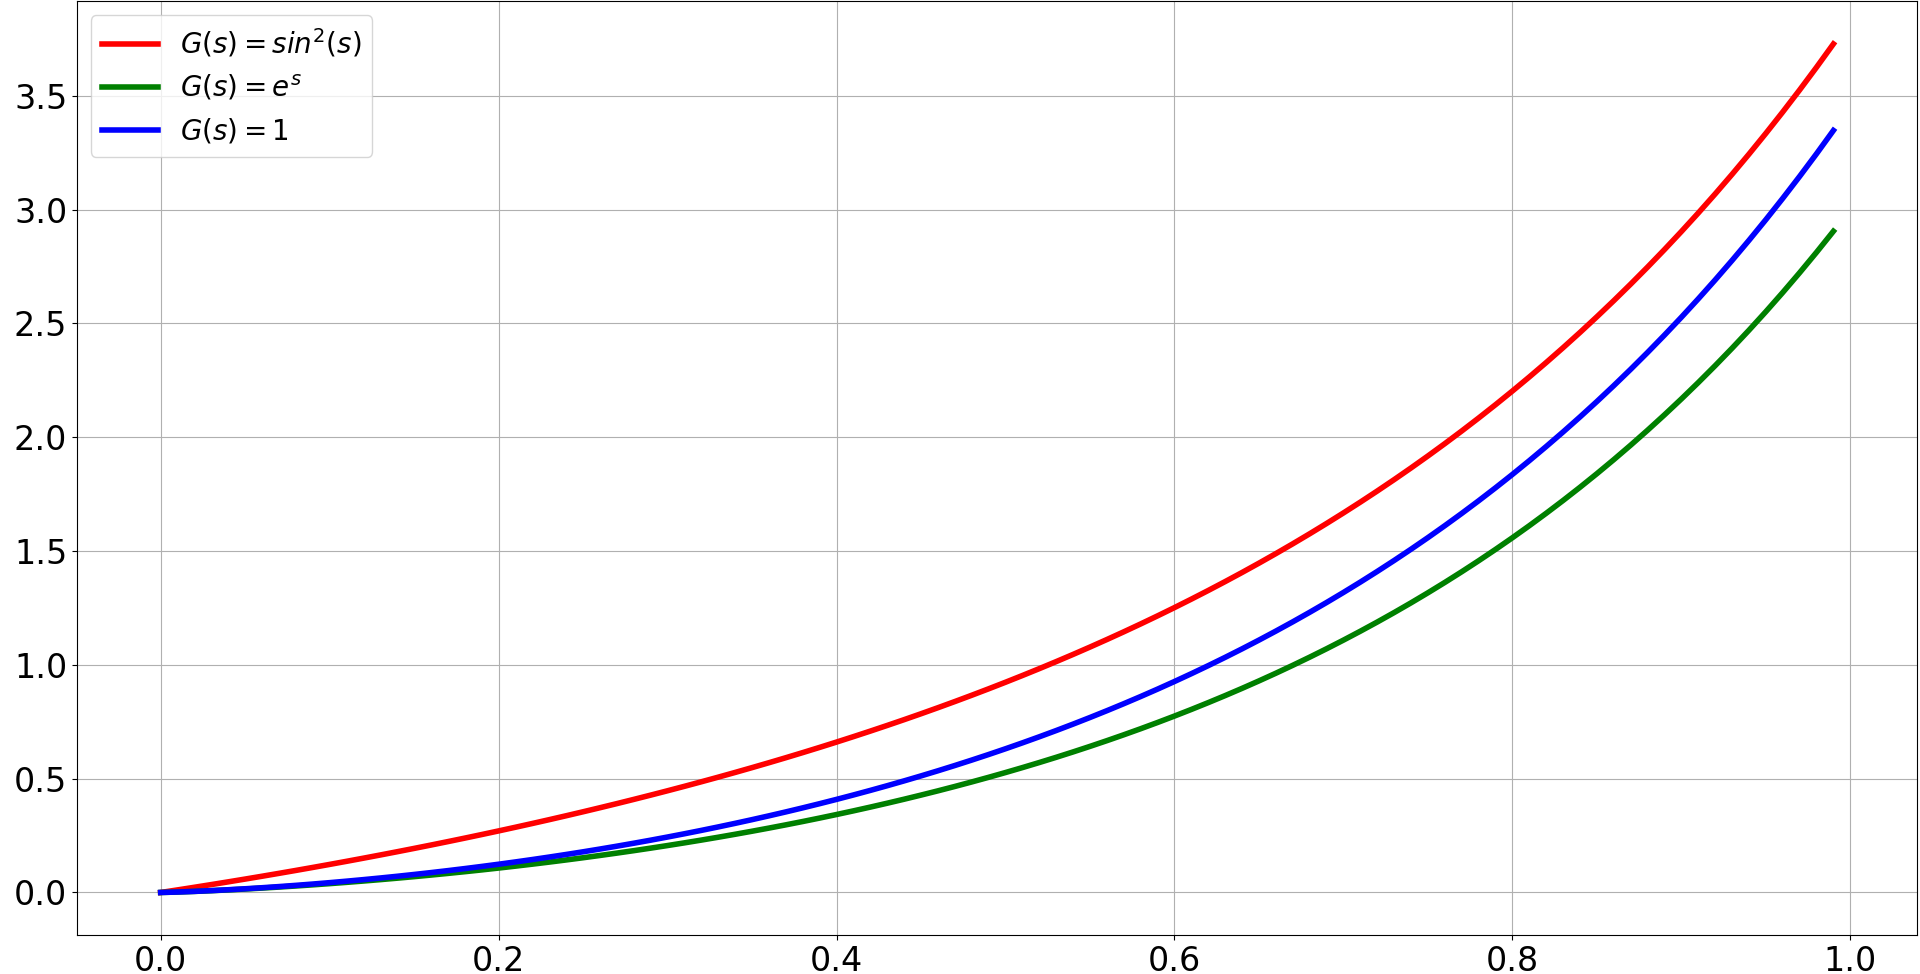
\includegraphics[width=1\linewidth]{plot}
    \caption{График функции (\ref{eq:C}) при $\norm{x_0} = 1$; $q = 0.5$; $d = 2$; $a = 1$; $T = 1$.}
    \label{fig:plot}
\end{figure}

Краткий алгоритм работы программы представлен ниже:

\begin{figure}[ht]
    \centering
    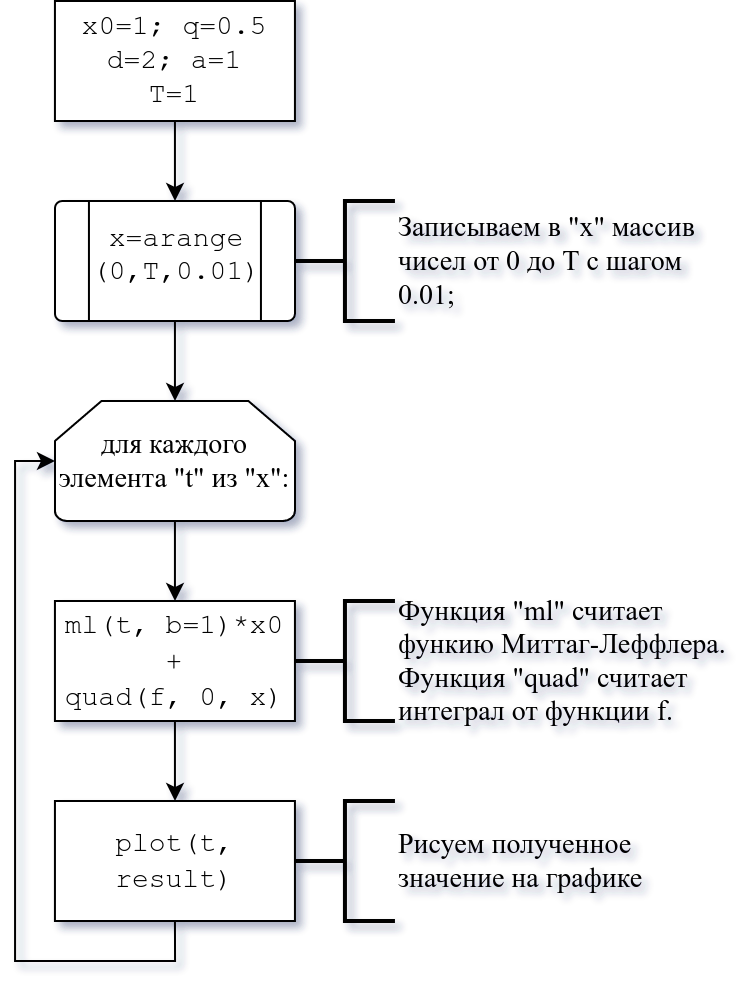
\includegraphics[width=0.35\linewidth]{diagram}
    \caption{Блок-схема программы.}
\end{figure}

\clearpage

\addcontentsline{toc}{section}{Список литературы}

\nocite{*}

\printbibliography{}

\clearpage

\section*{Приложение}
\addcontentsline{toc}{section}{Приложение}

\usemintedstyle{xcode}
\inputminted[fontfamily=courier, mathescape]{python}{app/main.py}
